\documentclass[bachelor, och, referat, times]{SCWorks}

% параметр - тип обучения - одно из значений:
%    spec     - специальность
%    bachelor - бакалавриат (по умолчанию)
%    master   - магистратура
% параметр - форма обучения - одно из значений:
%    och   - очное (по умолчанию)
%    zaoch - заочное
% параметр - тип работы - одно из значений:
%    referat    - реферат
%    coursework - курсовая работа (по умолчанию)
%    diploma    - дипломная работа
%    pract      - отчет по практике
%    pract      - отчет о научно-исследовательской работе
%    autoref    - автореферат выпускной работы
%    assignment - задание на выпускную квалификационную работу
%    review     - отзыв руководителя
%    critique   - рецензия на выпускную работу
% параметр - включение шрифта
%    times    - включение шрифта Times New Roman (если установлен)
%               по умолчанию выключен 


\usepackage[colorlinks=false, pdfborder={0 0 0}]{hyperref}  % убирает и цвет, и рамки
\usepackage[T2A]{fontenc}
\usepackage[utf8]{inputenc}
\usepackage[english,russian]{babel}
\usepackage{graphicx}
\usepackage[sort,compress]{cite}
\usepackage{amsmath}
\usepackage{amssymb}
\usepackage{amsthm}
\usepackage{fancyvrb}
\usepackage{longtable}
\usepackage{array}
\usepackage{minted}
\usepackage{tempora}
\usepackage{listings}
\usepackage{verbatim}



\newcommand{\eqdef}{\stackrel {\rm def}{=}}
\newcommand{\No}{\textnumero}
\newtheorem{lem}{Лемма}
\setminted{style=bw,
	linenos=true,
	breaklines=true,
	numbersep=5pt,
	tabsize=2,
	fontsize=\small,
	bgcolor=white}
\setmintedinline{style=bw,
	bgcolor=white,
	fontsize=\normalsize
	}
%убирание преносов слов
\tolerance = 1
\emergencystretch = \maxdimen
\hbadness = 10000

\newcommand{\eqdef}{\stackrel {\rm def}{=}}

\newtheorem{lem}{Лемма}

\begin{document}
    
   % Кафедра (в родительном падеже)
    %\chair{математической кибернетики и компьютерных наук}
    \chair{информатики и программирования}
    % Тема работы
    \title{Отчет по по предмету - "Структуры данных и алгоритмы".Задание 2.}
    
    % Курс
    \course{2}
    
    % Группа
    \group{211}
    
    % Факультет (в родительном падеже) (по умолчанию "факультета КНиИТ")
    \department{факультета компьютерных наук и информационных технологий}
    
    % Специальность/направление код - наименование
    
    \napravlenie{02.03.02 "--- Фундаментальная информатика и информационные технологии}
    
    % Для студентки. Для работы студента следующая команда не нужна.
    \studenttitle{студентки}
    
    % Фамилия, имя, отчество в родительном падеже
    \author{Никитенко Яны Валерьевны}
    
    % Заведующий кафедрой 
    %\chtitle{доцент, к.\,ф.-м.\,н.}
    %\chname{С.\,В.\,Миронов}
    % Научный руководитель (для реферата преподаватель проверяющий работу)
    %\satitle{доцент, к.\,ф.-м.\,н.} %должность, степень, звание
    %\saname{А.\,П.\,Грецова}
    % Руководитель ДПП ПП для цифровой кафедры (перекрывает заведующего кафедры)
    % \chpretitle{
    %     заведующий кафедрой математических основ информатики и олимпиадного\\
    %     программирования на базе МАОУ <<Ф"=Т лицей №1>>
    % }
    % \chtitle{г. Саратов, к.\,ф.-м.\,н., доцент}
    % \chname{Кондратова\, Ю.\,Н.}
    \date{2025}
    
    
    % Руководитель практики от организации (руководитель для цифровой кафедры)
    %\patitle{доцент, к.\,ф.-м.\,н.}
    %\paname{С.\,В.\,Миронов}
    
    % Руководитель НИР
    %\nirtitle{доцент, к.\,п.\,н.} % степень, звание
    %\nirname{В.\,А.\,Векслер}
    
    % Семестр (только для практики, для остальных типов работ не используется)
    %\term{2}
    
    % Наименование практики (только для практики, для остальных типов работ не
    % используется)
    %\practtype{учебная}
    
    % Продолжительность практики (количество недель) (только для практики, для
    % остальных типов работ не используется)
    %\duration{2}
    
    % Даты начала и окончания практики (только для практики, для остальных типов
    % работ не используется)
    %\practStart{01.07.2022}
    %\practFinish{13.01.2023}
    
    % Год выполнения отчета
   
    
    \maketitle

    
    % Включение нумерации рисунков, формул и таблиц по разделам
    % (по умолчанию - нумерация сквозная)
    % (допускается оба вида нумерации)
    %\secNumbering

    
    
   
    
    % Раздел "Обозначения и сокращения". Может отсутствовать в работе
    %\abbreviations
    %\begin{description}
    %    \item $|A|$  "--- количество элементов в конечном множестве $A$;
    %    \item $\det B$  "--- определитель матрицы $B$;
    %    \item ИНС "--- Искусственная нейронная сеть;
    %    \item FANN "--- Feedforward Artifitial Neural Network
    %\end{description}
    
    % Раздел "Определения". Может отсутствовать в работе
    %\definitions
    
    % Раздел "Определения, обозначения и сокращения". Может отсутствовать в работе.
    % Если присутствует, то заменяет собой разделы "Обозначения и сокращения" и "Определения"
    %\defabbr
    

    \textbf{Таблица} 

\begin{figure}[H]
    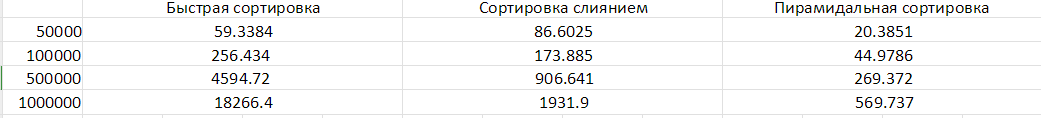
\includegraphics[width=1\linewidth]{Снимок экрана 2025-04-08 222327.png}
    \caption{Таблица}

    Время указано в милисекунднах
\end{figure}

\textbf{Графики} 
\begin{figure}[H]
    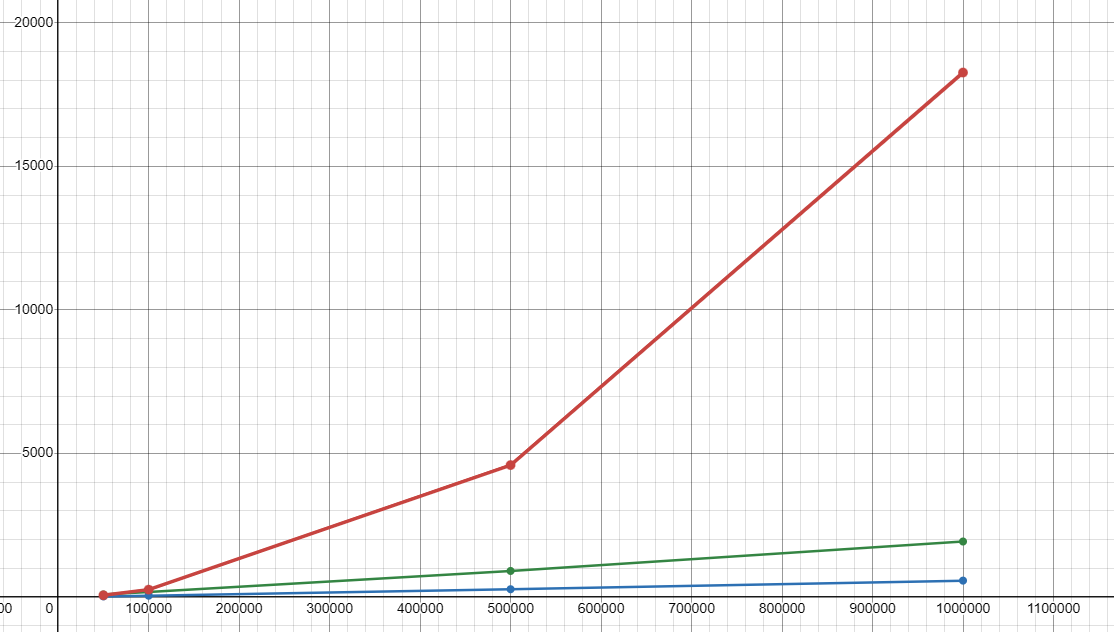
\includegraphics[width=1\linewidth]{Снимок экрана 2025-04-08 223347.png}
    \caption{Красная линия - Бытсрая сортировка
    Зеленая линия - Сортровка слияннием
    Синия линия - Пирамидальная сортировка}
\end{figure}

Самой медленной сортировкой оказалась быстрая. 
Самой быстрой же оказалась пирамидальная. 
По середине расположилась слияние. 


    \appendix
     
\end{document}